% Target-anchored computational prioritization of African-NP-inspired antimalarial candidates
% Target-anchored computational article — August 2026
\documentclass[journal=jcisd8,manuscript=article]{achemso}
\usepackage{amsmath,amssymb,mathtools}
\usepackage[T1]{fontenc}
\usepackage[utf8]{inputenc}
\usepackage{lmodern}
\usepackage[detect-all=true,group-minimum-digits=4]{siunitx}
\DeclareSIUnit\angstrom{\text{\AA}}
\DeclareSIUnit\dalton{Da}
\DeclareSIUnit\calorie{cal}
\usepackage{graphicx}
\usepackage{booktabs,tabularx,array,multirow}
\usepackage{xr}
\usepackage[colorlinks=true,linkcolor=blue,citecolor=blue,urlcolor=blue]{hyperref}
\usepackage[noabbrev,capitalize]{cleveref}
\externaldocument[SM-]{Antimalarial_Candidates_African_NP_V2608_SM}
\graphicspath{{Graphics/}}

\author{Myke Vital Sao Temgoua}
\email{myke-vital.sao@facsciences-uy1.cm}
\affiliation{Department of Physics, Faculty of Science, University of Yaoundé I, P.O. Box 812, Yaoundé, Cameroon}
\author{Jean-Pierre Tchapet Njafa}
\affiliation{Department of Physics, Faculty of Science, University of Yaoundé I, P.O. Box 812, Yaoundé, Cameroon}
\author{Penabei Samafou}
\affiliation{Department of Medical Imaging and Radiation Sciences, Faculty of Medicine and Health Sciences, Université de Sherbrooke, Sherbrooke, QC J1H 5N4, Canada}
\author{Wilfred Fon Mbacham}
\affiliation{Department of Biochemistry, Faculty of Science, University of Yaoundé I, P.O. Box 812, Yaoundé, Cameroon}
\author{Serge Guy Nana Engo}
\affiliation{Department of Physics, Faculty of Science, University of Yaoundé I, P.O. Box 812, Yaoundé, Cameroon}
\title{Target-Anchored Computational Prioritization of African-Natural-Product-Inspired Antimalarial Candidates}
\SectionNumbersOn
\begin{document}
\maketitle

\begin{abstract}
Polypharmacology is attractive in antimalarial discovery because simultaneous engagement of resistance-relevant proteins could reduce the probability that a single parasite mutation abolishes activity. We report a target-anchored computational analysis of a locked 17-member polypharmacology-oriented cohort derived from an African-natural-product-inspired chemical-space funnel. Each candidate was docked with AutoDock Vina against four \textit{Plasmodium falciparum} proteins: PfDHFR (7F3Y), PfCRT (6UKJ), PfClpP (2F6I), and PfATP4 (9N10). Pocket definitions were tied to a catalytic-site ligand, a membrane-proxy cavity, a catalytic triad, or conserved ATPase machinery, respectively, rather than to receptor centroids. All \num{68} candidate--target calculations passed a predeclared geometric gate requiring a rank-1 pose inside the search region, contact with the target-specific anchor, and at least \qty{90}{\percent} of ligand atoms inside the padded box. Docking-score estimates ranged from \qtyrange{-7.91}{-4.63}{\kilo\calorie\per\mole}; target-wise means were \num{-5.755} (PfDHFR), \num{-6.185} (PfCRT), \num{-5.935} (PfClpP), and \num{-6.308} (PfATP4). These target-wise summaries are not combined across pockets. The results support a reproducible, target-anchored pose-prioritization workflow, not experimental affinity, target engagement, or resistance circumvention. The complete candidate-level table and structural provenance are provided as machine-readable supplementary data.\end{abstract}

\noindent\textbf{Keywords:} antimalarial drug discovery; African natural products; polypharmacology; molecular docking; PfDHFR; PfCRT; PfClpP; PfATP4

\section{Introduction}
Malaria remains a major infectious-disease burden, and the spread of resistance motivates antimalarial strategies that do not depend on a single vulnerable molecular interaction. Target-based discovery can provide mechanistic hypotheses, but docking scores are sensitive to receptor preparation, pocket definition, ligand protonation, and search-space geometry \cite{kitchen2004,Simoben2023}. A computational screen is therefore most useful when it states precisely what is being tested and separates pose compatibility from biological validation.

Natural-product-inspired chemical space is a productive source of antimalarial hypotheses because its scaffolds span structural complexity that is often under-represented in conventional synthetic libraries. In the preceding chemical-space funnel, African natural products were combined with synthetic antimalarial chemistry, expanded by similarity and SELFIES-based perturbation, and filtered for novelty, drug-likeness, and synthetic tractability. That funnel produced a set of candidates with predicted multi-target profiles. The present study addresses the next methodological question: can a fixed polypharmacology-oriented cohort be evaluated against biologically motivated pockets without conflating docking geometry with measured activity?

We selected four resistance-relevant proteins with complementary biological roles: dihydrofolate reductase (PfDHFR), the chloroquine resistance transporter (PfCRT), the caseinolytic protease subunit PfClpP, and the P-type ATPase PfATP4. The structures do not provide equivalent evidence. PfDHFR contains a catalytic-site methotrexate copy; PfCRT contains a membrane-associated Y01 cavity proxy; PfClpP contains a resolved catalytic triad; and the PfATP4 structure provides conserved catalytic machinery but no co-crystallized small-molecule inhibitor. We therefore use target-specific anchors and report the evidence class of each pocket.

Our hypothesis was deliberately limited: target-anchored docking would yield a reproducible four-target pose matrix suitable for prioritizing candidates and for later resistance-resilience analysis. We did not hypothesize that a docking score is an affinity measurement or that a four-target computational profile proves polypharmacological efficacy.

\section{Materials and Methods}
\subsection{Candidate cohort and chemical-space funnel}
The starting workflow combined \num{396} African natural products with \num{454} synthetic antimalarial compounds. Similarity-based expansion and SELFIES perturbation generated a deduplicated hybrid library of \num{65856} molecules. A variational autoencoder representation, clustering, multi-parameter optimization, and synthetic-accessibility filtering produced a prioritized lead space. The present analysis used the prespecified 17-member polypharmacology-oriented cohort (Set C), whose canonical SMILES and source hash are provided in the candidate manifest. This cohort is distinct from the MPO top-20 set and from the four parent systems used in the historical MD study.

\subsection{Target structures and biological anchors}
The receptor files were prepared as protein-only structures, retaining the coordinate frame used for the target-specific pocket definition. The four anchors were:
\begin{itemize}
\item PfDHFR, PDB 7F3Y: the catalytic-site methotrexate copy A702, whose contacts include canonical active-site residues;
\item PfCRT, PDB 6UKJ: the Y01-associated cavity in chain A, treated as a membrane/cavity proxy rather than an inhibitor site;
\item PfClpP, PDB 2F6I: chain-A Ser252/His223/Asp219 catalytic triad; PDB 4GM2 was excluded because it is PfClpR, not PfClpP;
\item PfATP4, PDB 9N10: the conserved P-type ATPase region around the phospho-site D451 and the A-domain DPPR hinge. Because no small-molecule inhibitor is co-crystallized, this is a mechanism-motivated region rather than a pocket validated by a co-crystallized small-molecule ligand.
\end{itemize}
The anchor coordinates, receptor hashes, and pocket evidence classes are listed in Supplementary \Cref{SM-tab:anchors}.

\subsection{Ligand preparation and docking}
SMILES were standardized and converted to three-dimensional ligand structures with explicit protonation and rotatable-bond records. Ligand PDBQT files were generated with Meeko. AutoDock Vina was run independently for each candidate--target pair using fixed target-specific boxes and target-specific exhaustiveness settings, following established docking practice \cite{Trott2009,Eberhardt2021}. No post hoc translation of poses or expansion of boxes was permitted. The docking score is reported in \si{\kilo\calorie\per\mole} and is interpreted only as a Vina scoring-function estimate.

\subsection{Predeclared geometric gate and provenance}
A pair was classified as geometrically admissible when (i) the rank-1 pose centroid was inside the declared search box, (ii) at least one ligand atom was within \qty{10}{\angstrom} of the target-specific anchor atoms, and (iii) at least \qty{90}{\percent} of ligand atoms were inside the box with the declared padding. This geometric criterion tests computational placement, not binding. For every pair, the supplementary record stores the receptor, ligand, configuration, output pose, conversion log, and hashes. Automated integrity checks are reported as reproducibility controls and are not interpreted as biological validation.

\subsection{Summary statistics}
For each target we report the range and mean of the 17 Vina scores, the proportion of pairs passing the geometric gate, and the range of anchor distances. We did not compute a four-target consensus score, an RRS value, or a PNS value from this panel because those analyses require the separate cohort-level review and mutation definitions described in the integrated study.

\section{Results}
\subsection{A chemically diverse, fixed polypharmacology-oriented cohort}
The 17 candidates were retained as a locked cohort rather than selected after inspecting the corrected docking scores. Their structures span flavonoid, coumarin, alkaloid-like, lignan-like, and terpenoid-inspired chemotypes. This design prevents the target panel from being used as a post hoc enrichment exercise and permits a direct candidate-by-target comparison.

\subsection{Target-anchored docking produces a complete pose matrix}
All \num{68} candidate--target pairs passed the predeclared geometric gate. The target-specific score ranges were \qtyrange{-6.35}{-4.86}{\kilo\calorie\per\mole} for PfDHFR, \qtyrange{-7.91}{-5.12}{\kilo\calorie\per\mole} for PfCRT, \qtyrange{-7.03}{-5.05}{\kilo\calorie\per\mole} for PfClpP, and \qtyrange{-7.57}{-4.63}{\kilo\calorie\per\mole} for PfATP4. The corresponding target-wise means were \num{-5.755}, \num{-6.185}, \num{-5.935}, and \num{-6.308}, respectively. These summaries are kept separate because Vina scores are not calibrated across unlike receptor pockets. Candidate-level values are given in Supplementary \Cref{SM-tab:vina_matrix}.

The most favorable within-target estimates included PP-06 in the PfCRT cavity (\num{-7.91}) and PP-13 in the PfATP4 machinery region (\num{-7.57}). These observations are descriptive within each target and are not a cross-target potency ranking: the pockets have different evidence classes, and Vina scores are not calibrated across targets. The complete candidate-by-target matrix is therefore retained without a composite score. The target-wise distributions and candidate-level ordering are visualized in \Cref{fig:targetwise}; the corresponding rank and gate-quality displays are provided in Supplementary \Cref{SM-fig:rank,SM-fig:qc}.

\begin{figure}[htbp]
\centering
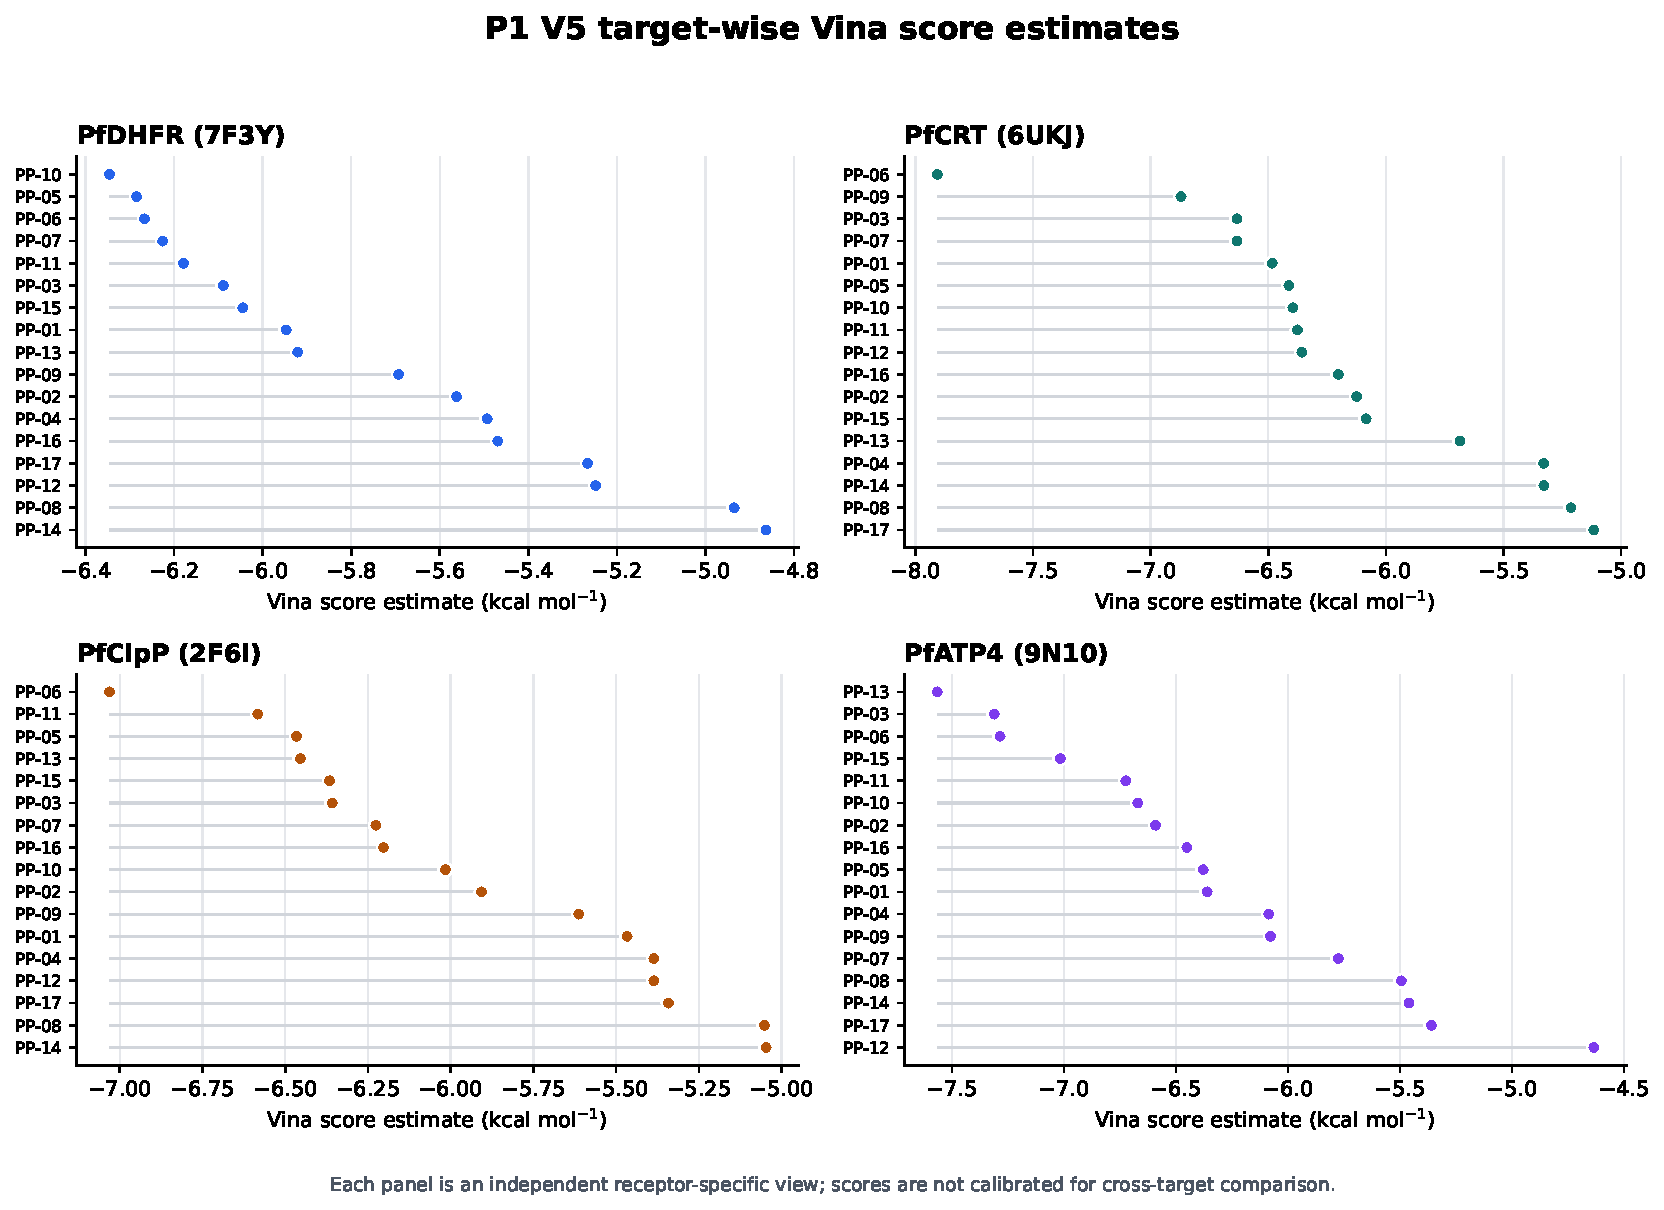
\includegraphics[width=\textwidth]{p1_v5_targetwise_vina_scores.pdf}
\caption{Target-wise Vina score estimates for the locked 17-member cohort. Each panel is an independent receptor-specific view, ordered from the most negative to the least negative score within that target. Scores are AutoDock Vina scoring-function outputs and are not calibrated for cross-target comparison; the figure does not represent a four-target potency ranking. The panel is computational evidence and does not constitute biological validation.}
\label{fig:targetwise}
\end{figure}

\subsection{Pocket evidence determines the interpretation of the matrix}
The complete geometric pass rate should not be mistaken for equivalent biological support across targets. PfDHFR and PfClpP use chemically meaningful catalytic-site anchors; PfCRT is relative to a membrane-associated proxy cavity; and PfATP4 is relative to conserved catalytic machinery in a structure without a co-crystallized inhibitor. Accordingly, the matrix is best interpreted as a standardized hypothesis-generation layer. It identifies candidate--pocket configurations that merit orthogonal testing, while preserving the uncertainty associated with the underlying structural evidence.

\section{Discussion}
This study converts a broad African-natural-product-inspired prioritization problem into a reproducible candidate-by-target pose matrix. The central methodological result is not that all 17 candidates are binders, but that target-specific biological anchors can be defined explicitly and audited before scores are compared. The distinction is particularly important for membrane proteins and large catalytic assemblies, for which a receptor centroid is not a defensible proxy for a ligand site.

The four-target matrix creates a useful interface with resistance-resilience analysis. A polypharmacology profile describes the breadth of predicted target-compatible poses; RRS, in contrast, requires a target-specific mutant panel and a non-binding-aware denominator. These are complementary analyses, not interchangeable metrics. The present article therefore reports the docking layer without manufacturing an RRS conclusion from the 68 wild-type scores.

Several limitations bound the interpretation. Vina scores are approximate scoring-function outputs and are not experimental binding free energies. The Y01-associated PfCRT cavity is a membrane proxy, and the PfATP4 region is mechanism-motivated rather than inhibitor-anchored. Rigid-receptor docking does not capture induced fit, membrane dynamics, protonation uncertainty, or solvent reorganization. The 17-member cohort was not an external prospective benchmark, and no IC\textsubscript{50}/EC\textsubscript{50} measurements were available for this analysis. Finally, the automated integrity record does not replace independent structural review. These limitations motivate biochemical binding measurements, cellular antimalarial assays, mutant-panel testing, and molecular-dynamics or free-energy calculations on a small number of experimentally tractable candidates.

\section{Conclusion}
A target-anchored Vina workflow generated a complete 17-by-4 computational pose matrix for an African-natural-product-inspired polypharmacology-oriented cohort. The workflow corrected a target-identity error by using PfClpP structure 2F6I rather than PfClpR structure 4GM2, distinguished ligand-anchored, proxy, and machinery-motivated pockets, and preserved raw pose provenance. The resulting candidates are computational hypotheses for multi-target and resistance-resilience studies, not confirmed inhibitors. The associated RRS and polypharmacology interpretation is developed separately using a per-target mutation-aware definition.

\section*{Supporting Information}
The Supporting Information contains target-anchor definitions, the complete 17-by-4 score matrix, per-pair geometric metrics, ligand-preparation details, receptor and configuration hashes, and the data dictionary for the machine-readable review table.

\section*{Author Contributions}
M.V.S.T. and S.G.N.E. designed the computational study. M.V.S.T. and J.-P.T.N. developed the chemical-space and docking workflow. P.S. and W.F.M. contributed to biological interpretation. All authors reviewed the manuscript and approved its scientific scope.

\section*{Notes}
The authors declare no competing financial interest. All interpretations are computational and hypothesis-generating.

\section*{Data Availability}
Canonical SMILES, target structures, ligand files, raw Vina outputs, configuration files, hashes, and analysis scripts are available in the project repository: \url{https://github.com/NanaEngo/Malaria_codesV2}. The machine-readable four-target table is \texttt{results/v5\_four\_target\_vina\_review\_table.json}. The dataset and its computational limitations are described alongside the machine-readable results.

\bibliography{../bibliography/Sao_Chim_Space}
\end{document}
